\documentclass[10pt]{beamer}
\usetheme[progressbar=frametitle]{metropolis}
\usepackage{booktabs, color}
\usepackage[scale=2]{ccicons}
\usepackage{natbib}
\bibliographystyle{unsrtnat}
\usepackage{pgfplots}
\usepgfplotslibrary{dateplot}
\usepackage{amsmath}
\usepackage{xspace}
\newcommand{\themename}{\textbf{\textsc{metropolis}}\xspace}
\usepackage{CJKutf8}
\newcommand\lheq{\stackrel{\mathclap{\normalfont\mbox{L'H}}}{=}}
\setbeamertemplate{theorem begin}{%
%  \begin{\inserttheoremblockenv}% removed
  {%
    \textcolor{blue}{\inserttheoremname\space\inserttheoremnumber.}
    \ifx\inserttheoremaddition\else\ \fi%
    % new
  }%
}
\setbeamertemplate{theorem end}{}
\makeatletter
\newenvironment<>{proofs}[1][\proofname]{%
    \par
    \def\insertproofname{#1\@addpunct{.}}%
    \usebeamertemplate{proof begin}#2}
  {\usebeamertemplate{proof end}}
\newenvironment<>{proofc}{%
  \setbeamertemplate{proof begin}{\begin{block}{}}
    \par
    \usebeamertemplate{proof begin}}
  {\usebeamertemplate{proof end}}
\newenvironment<>{proofe}{%
    \par
    \pushQED{\qed}
    \setbeamertemplate{proof begin}{\begin{block}{}}
    \usebeamertemplate{proof begin}}
  {\popQED\usebeamertemplate{proof end}}
\makeatother
\begin{CJK*}{UTF8}{bsmi}
\title{A Law of Iterated Logarithm for Reflected Fractional Brownian Motion}

\date{August 21, 2020}
\author{Simon Chung\\ Advising Professor:May-Ru Chen}
\institute{Department of Applied Mathematics, \\National Sun Yat-sen University }
\titlegraphic{\hfill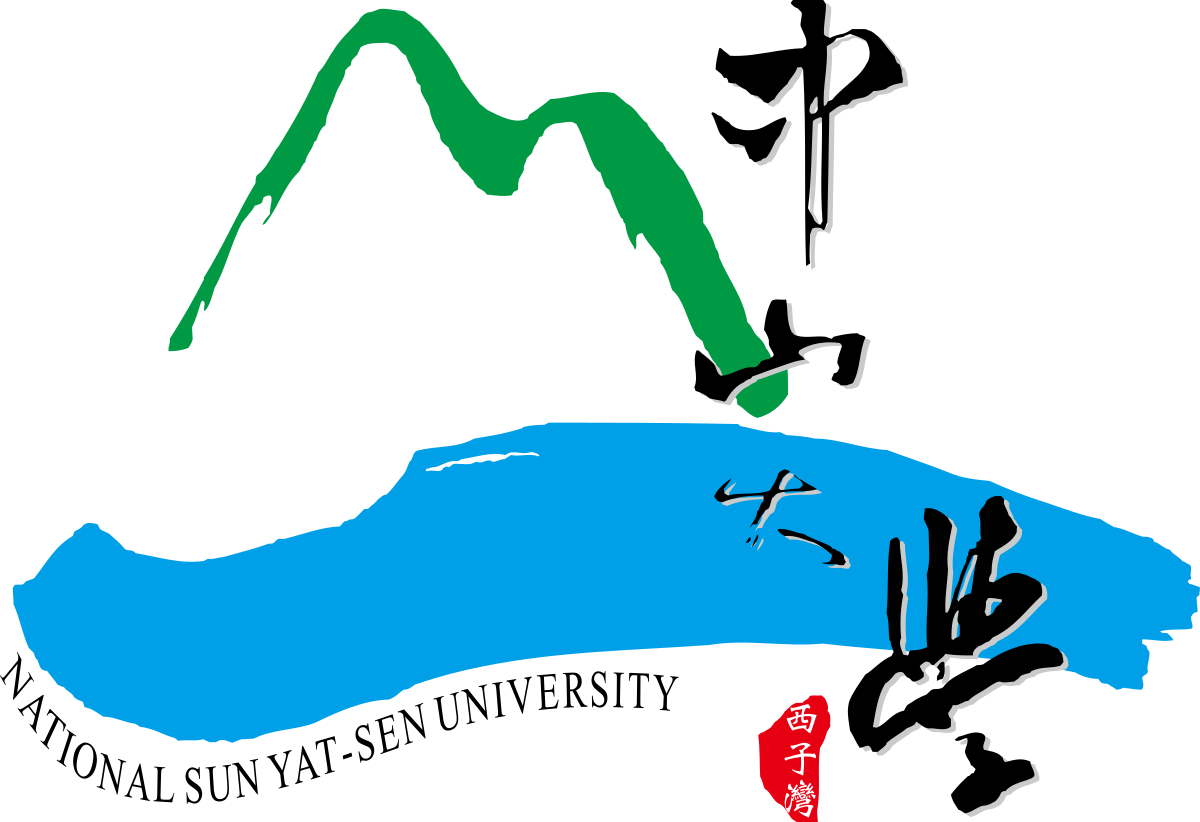
\includegraphics[height=1.3cm]{nsysu_logo.png}}



\begin{document}

\maketitle

\begin{frame}{Table of Contents} 
  \setbeamertemplate{section in toc}[sections numbered]
  \tableofcontents%[hideallsubsections]
\end{frame}


%==========================================================================================================
\section{Introduction}

%--- Gaussian process ---------------------------------------------------------------------------------------------
\begin{frame}[fragile]{Gaussian Process}  \transwipe[direction=0]  %製作換頁效果
The stochastic process $\{X(t),\,t\in\mathbb{T}\}$ is called a {\color{blue} Gaussian process} if
\\for any $m\geqslant1$ and any points $\{t_1,...,t_m\}\subset\mathbb{T}$,
the vector $\left(X(t_1),...,X(t_m)\right)$ follows a multivariate normal distribution.
\end{frame}

%----- Brownain motion -----------------------------------------------------------------------------------------
\begin{frame}[fragile]{Brownain Motion}
\vspace{0.5cm}
Let $B = \{B(t):t \in \mathbb{R_+} \}$ be a {\color{blue} standard Brownain motion}, which satisfied the following properties.
\begin{itemize}
		\item[(i)] $B(0)=0$ almost surely;
		\item[(ii)] $B$ has stationary independent increments and $B(t)-B(s)\sim \mathcal{N}(0, t-s)$ for $0\leq s < t$;
		\item[(iii)] almost surely, the paths of $B$ are continuous.
	\end{itemize}
	
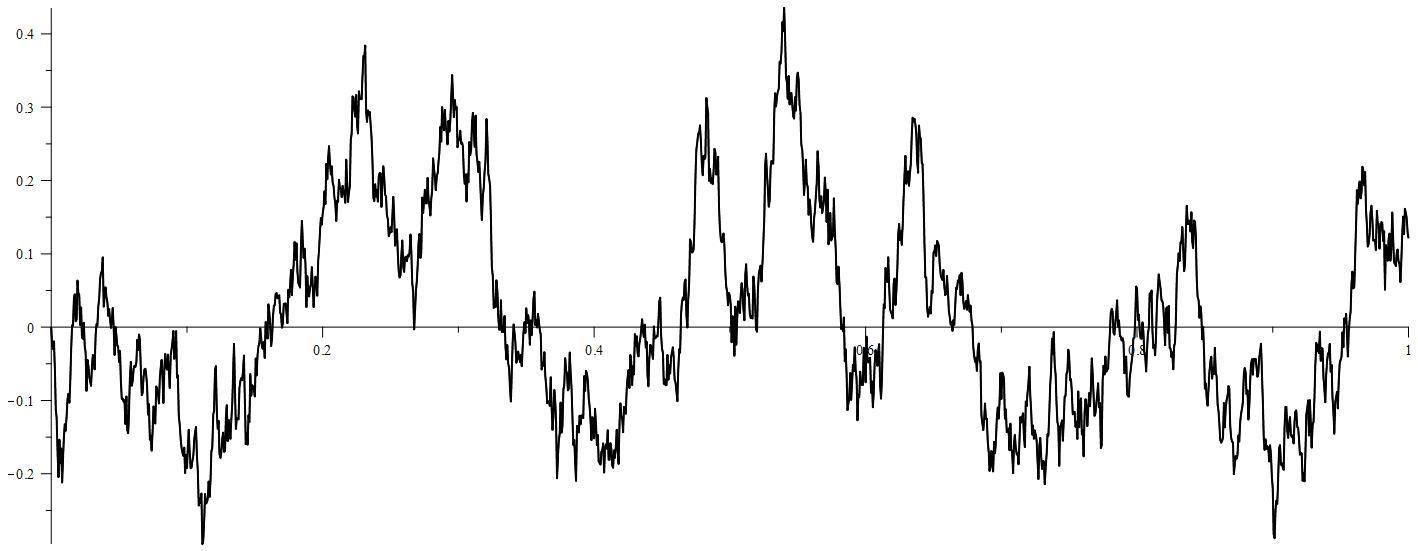
\includegraphics[width=1\linewidth, height=3.5cm]{BM.JPG}
\end{frame}


%-----fractional Brownian motion ---------------------------------------------------------------------------------
\begin{frame}[fragile]{Fractional Brownian Motion}
Let $B_H = \{B_H(t):t \in \mathbb{R}_+ \}$ be a {\color{blue} standard fractional Brownian motion} (fBm) with Hurst parameter $H \in (0,1)$, which defined as a centered Gaussian process with covariance function
$$\mbox{Cov}(B_H(t),B_H(s)) = \frac{1}{2}\left(|t|^{2H}+|s|^{2H}-|t-s|^{2H}\right).$$

\pause
Note that \\
(i) if $H = \frac{1}{2}$, then $B_H$ is the standard Brownian motion $B$;\\

\pause
(ii) fBm is selfsimilar, i.e., $\{B_H(t),\, t\in\mathbb{R}_+\}$ and $\{s^{-H}B_H(st),\, t\in\mathbb{R}_+\}$ have the sane distribution for any $s>0$.
\end{frame}

%-------------------------------------------------------------------------------------------------------------
\begin{frame}[fragile]{Reflected Fractional Brownian Motion}
Consider a {\color{blue} reflected (at 0) fractional Brownian motion} (rfBm) with drift $Q_{B_{H}}= \{B_H(t):t \in \mathbb{R_+} \}$, given by the following formula
$$Q_{B_{H}}(t)=B_H(t)-ct+\max\left(Q_{B_{H}}(0),-\inf\limits_{s\in [0,t]}(B_H(s)-cs)\right),$$
where $c>0$.
To simplify the notation, we assume $c = 1$ in this talk.

\pause
Note that if $Q_{B_{H}}(0)=0$, then
$$
Q_{B_{H}}(t)
=B_H(t)-ct-\inf\limits_{s\in [0,t]}(B_H(s)-cs)
=\sup_{-\infty<s\leq t}(B_H(t)-B_H(s)-c(t-s))
$$
\end{frame}


%==========================================================================================================
\section{Literature Review}
\begin{frame}[label=table]{Literature Review}  \transwipe[direction=0]  %製作換頁效果
\newcommand{\dis}{\displaystyle}
$$\begin{tabular}{|l|c|c|c|}
    \hline
    \mbox{Form} & $\dis\frac{B(t)}{\sqrt{2t\ln\ln t}}$
                & $\dis\frac{\max_{0\leq s\leq t}|B(s)|}{\sqrt{2t\ln\ln t}}$
                & $\dis\frac{\max_{0\leq s\leq t}|B(s)|}{\sqrt{t/\ln\ln t}}$\\
                \hline
    $\limsup_{t\nearrow \infty}$ &  {\color{blue} \hyperlink{BMLIL}{1}} & \hyperlink{MBMLIL}{1} &  $\times$                    \\
    \hline
    $\liminf_{t\nearrow \infty}$ & {\color{blue} \hyperlink{BMLIL}{-1}} & $\times$  & {\color{blue} $\hyperlink{MBMLIL}{\frac{\pi}{\sqrt{8}}}$}  \\
    \hline
    \mbox{Form} & $\dis\frac{B_{H}(t)}{\sqrt{2t^{2H}\ln\ln \frac{1}{t}}}$
                & $\dis\frac{\max_{0\leq s\leq t}|B_{H}(s)|}{\sqrt{2t^{2H}\ln\ln \frac{1}{t}}}$
                & $\dis\frac{\max_{0\leq s\leq t}|B_{H}(s)|}{\sqrt{(2t/\ln\ln t)^{2H}}}$\\
                \hline
    $\limsup_{t\nearrow 0}$ & 1  & {\color{blue} \hyperlink{MFBMLIL}{1}} & $\times$   \\
    \hline
    $\liminf_{t\nearrow 0}$ & -1 & $\times$ & {\color{blue} $\hyperlink{MFBMLIL}{c_\alpha}$} \\
    \hline
    \mbox{Form} & $\dis\frac{Q_{B_{H}}(t)}{(\frac{2}{A^2}\ln{t})^{\frac{1}{2(1-H)}}}$
                & $\dis\frac{\max_{0\leq s\leq t}Q_{B_{H}}(s)}{g(t)} $
                & $\dis\frac{\max_{0\leq s\leq t}Q_{B_{H}}(s)}{h(t)} $\\
                \hline
    $\limsup_{t\nearrow \infty}$ &$ \hyperlink{rfBmLIL}{1}$ & \hyperlink{MRFBMLIL}{?} & $\times$ \\
    \hline
    $\liminf_{t\nearrow \infty}$ & 0 & $\times$  & \hyperlink{MRFBMLIL}{?}\\
    \hline
  \end{tabular}$$
\end{frame}


\begin{frame}[label=BMLIL]{LIL for $B(t)$}
The Classic Law of Iterated Logarithm (LIL) is used to describe the the limit behavior of the fluctuations of standard Brownian motion, which has the form
$$\limsup\limits_{t\rightarrow 0} \frac{B(t)}{\sqrt{2t\ln{\ln{\frac{1}{t}}}}} = 1\;\mathrm{and}\; \limsup\limits_{t\rightarrow \infty} \frac{B(t)}{\sqrt{2t\ln{\ln{t}}}} = 1\quad \mathrm{a.s.}$$
Note that the denominator in the above equation is the maximum height of the fluctuation of $B$ above 0 as $t \to \infty$.
\\By the reflection principle for Brownian motion, we can easily acquire that
$$\liminf\limits_{t\rightarrow 0} \frac{B(t)}{\sqrt{2t\ln{\ln{\frac{1}{t}}}}} = -1\;\mathrm{and}\;\liminf\limits_{t\rightarrow \infty} \frac{B(t)}{\sqrt{2t\ln{\ln{t}}}} = -1 \quad \mathrm{a.s.}$$
\hfill\hyperlink{table}{\beamerbutton{table}}
\end{frame}

\begin{frame}[label=MBMLIL]{LIL for $\max_{0\leq s\leq t}|B(s)|$}
Next consider the cumulative maximum process of absolute Brownian motion.  The $\liminf_{t\to0}$ version was proved by \cite{chung1948maximum} and we can derivate the $\limsup_{t\to0}$ result.
$$\limsup\limits_{t\rightarrow 0} \frac{\max\limits_{s\leqslant t}|B(s)|}{\sqrt{2t\ln{\ln{\frac{1}{t}}}}} = 1 \; \mathrm{and}\;
\liminf\limits_{t\rightarrow 0} \frac{\max\limits_{s\leqslant t}|B(s)|}{\sqrt{t/\ln{\ln{t}}}} = \frac{\pi}{\sqrt{8}} \quad \mathrm{a.s.}$$
\hfill\hyperlink{table}{\beamerbutton{table}}
\end{frame}

\begin{frame}[label=MFBMLIL]{LIL for $\max_{0\leq s\leq t}|B_H(s)|$}
Next consider the cumulative maximum process of $|B_H|$. The $\limsup_{t\to0}$ result is shown in \cite{li2001gaussian} and the $\liminf_{t\to0}$ result is proved by \cite{monrad1995small}.
$$\limsup\limits_{t\rightarrow 0} \frac{\max\limits_{s\leqslant t}|B_{H}(t)|}{\sqrt{2t^{2H}\ln\ln\frac{1}{t}}} = 1 \; \mathrm{and}\;
\liminf\limits_{t\rightarrow 0} \frac{\max\limits_{s\leqslant t}|B_{H}(t)|}{t^{H}/(\ln\ln t)^H} = c_\alpha \quad \mathrm{a.s.},$$
where $c_\alpha$ is a positive constant.
\hfill\hyperlink{table}{\beamerbutton{table}}
\end{frame}



\begin{frame}[label=rfBmLIL]{LIL for $Q_{B_H}(t)$}
Recently, the LIL for rfBm is given in \cite{almostsurelyconvergence} without a clear proof.
\begin{theorem}
	\begin{align*}
		\limsup\limits_{t\rightarrow \infty} \frac{Q_{B_{H}}(t)}{(\frac{2}{A^2}\ln{t})^{\frac{1}{2(1-H)}}} = 1 \quad \mathrm{a.s.},
	\end{align*}
where $A = \frac{1}{1-H}(\frac{H}{1-H})^{-H}$.
\end{theorem}
\end{frame}

%==========================================================================================================
\section{The Proof of LIL for Reflected Fraction Brownian Motion}
\begin{frame}[fragile]{The Proof of LIL for rfBm}  \transwipe[direction=0]  %製作換頁效果
\begin{proofs}[Proof of Theorem 1]
\medskip
The proof can be separated into two parts, which is
\begin{equation}
	\mathbb{P}\left(\limsup\limits_{t\rightarrow \infty} \frac{Q_{B_{H}}(t)}{(\frac{2}{A^2}\ln{t})^{\frac{1}{2(1-H)}}}\geqslant1\right)=1
\end{equation}
and
\begin{equation}
	\mathbb{P}\left(\limsup\limits_{t\rightarrow \infty} \frac{Q_{B_{H}}(t)}{(\frac{2}{A^2}\ln{t})^{\frac{1}{2(1-H)}}}\leqslant1\right)=1.
\end{equation}
If we can prove that $\mathbb{P}\left(Q_{B_H}(t)<f(t)\quad\mathrm{i.o.}\right)=0$, then (1) will hold.
\\Similarly, (2) will hold if we can have $\mathbb{P}\left(Q_{B_H}(t)<f(t)\quad\mathrm{i.o.}\right)=1$.
\end{proofs}
\end{frame}
\begin{frame}[label=theorem2]{The Proof of LIL for rfBm}
Therefore, we need the following two Theorems.
\begin{theorem}
(\cite{almostsurelyconvergence}) For all positive and nondecreasing functions $f(t)$ on some interval $[T,\infty)$,
$$\mathbb{P}(Q_{B_{H}}(t)>f(t)\quad\mathrm{i.o.})=0\quad\mathrm{or}\quad1,$$
according as the integral
$$\mathcal{I}_f:=\int_T^\infty\frac{1}{f(u)}\mathbb{P}\left(\sup\limits_{t\in[0,f(u)]}Q_{B_{H}}(t)>f(u)\right)du $$
is finite or \hyperlink{halffinished}{infinite}.
\end{theorem}
\end{frame}

\begin{frame}[label=theorem3]{The Proof of LIL for rfBm}
\begin{theorem}
(\cite{piterbarg2001large}) For any $H\in(0,1)$, as $u\to\infty$
\begin{equation}
    \resizebox{\textwidth}{!}
     {%
$\mathbb{P}\left(\sup\limits_{[0,Tu]}Q_{B_{H}}(t)>u\right)=\sqrt{\pi}a^{\frac{2}{H}}b^{-\frac{1}{2}}T\mathcal{H}_{B_{H}}^2(Au^{1-H})^{\frac{2}{H}-1}\Psi(Au^{1-H})(1+o(1)),$%
	}
\end{equation}
where $$\tau_0 = \frac{H}{1-H}\;,a = \frac{1}{2\tau_{0}^{2H}}\;,B = H\left(\frac{H}{1-H}\right)^{-H-2}\;,b = \frac{B}{2A},$$
$$\mathcal{H}_{B_{H}}=\lim\limits_{T\to\infty}T^{-1}\mathbb{E}\exp\left(\sup\limits_{t\in[0,T]}(\sqrt{2}B_{H}(t)-t^{2H})\right)\in(0,\infty)$$
 and $\Psi(u)=\frac{1}{\sqrt{2\pi}}\int_{u}^{\infty}\exp(-\frac{1}{2}x^2)dx$.
\end{theorem}
\end{frame}


\begin{frame}[fragile]{The Proof of LIL for rfBm}
Let $T = 1$ and replace $u$ with $f_p(t)$ in (3), we see that as $u\to\infty$,
\begin{equation}
    \resizebox{\textwidth}{!}
     {%
		$\mathbb{P}\left(\sup\limits_{[0,f_p(u)]}Q_{B_{H}(t)}>f_p(u)\right)=\sqrt{\pi}a^{\frac{2}{H}}b^{-\frac{1}{2}}\mathcal{H}_{B_{H}}^2(Af_p(u)^{1-H})^{\frac{2}{H}-1}\Psi(Af_p(u)^{1-H})(1+o(1)).$%
		}
\end{equation}
\pause
To calculate (4), let 
$$g(u) = \ln{u} + (1+c_H-p)\ln{\ln{u}}\;\;\mathrm{and}\;\;f_p(u)= (2A^{-2}g(u))^{\frac{1}{2(1-H)}},$$
where $c_H = \frac{1}{H}-1-\frac{1}{2(1-H)}$.
\\Notice that for all $p\in\mathbb{R}$, $g(u)\to\infty$ implies $f(u)\to\infty$ as $u\to\infty$.
\end{frame}
\begin{frame}[fragile]{The Proof of LIL for rfBm}
From (2), there exists $u_1$ large enough such that for all $u>u_1$,
$$I(u)=\frac{1}{f_p(u)}\mathbb{P}\left(\sup\limits_{[0,f_p(u)]}Q_{B_{H}}(t)>f_p(u)\right)=
C\frac{\Psi(\sqrt{2g(u)})}{g(u)^{-(c_H+\frac{1}{2})}}$$
where $C=2^{c_H+\frac{1}{2}}\sqrt{\pi}A^{\frac{1}{1-H}}a^{\frac{2}{H}}b^{-\frac{1}{2}}\mathcal{H}^2_{B_{H}}(1+o(1))$.
\end{frame}

\begin{frame}[fragile]{The Proof of LIL for rfBm}
Since
$$\lim\limits_{t\to\infty}\frac{\Psi\left(\sqrt{2t}\right)}{\frac{1}{\sqrt{4\pi t}}\exp(-t)}\lheq\lim\limits_{t\to\infty}\frac{t^{-\frac{1}{2}}}{\frac{1}{2}t^{-\frac{3}{2}}+t^{-\frac{1}{2}}}=1,$$
there exists $u_2\geqslant u_1$ large enough such that for $u\geqslant u_2$,
$$\Psi(\sqrt{2t})=\frac{1}{\sqrt{4\pi t}}\exp(-t)\left(1+o(1)\right).$$
\end{frame}
\begin{frame}[fragile]{The Proof of LIL for rfBm}
Recall $g(u) = \ln{u} + (1+c_H-p)\ln{\ln{u}}$.
\\For any $p\in\mathbb{R}$ and $u>u_2$,

\begin{align*}
I(u)&=C\frac{\Psi(\sqrt{2g(u)})}{g(u)^{-(c_H+\frac{1}{2})}}
=\mathcal{C}\frac{\frac{1}{\sqrt{2\pi}}\frac{1}{\sqrt{2g(u)}}\exp(-g(u))\left(1+o(1)\right)}{g(u)^{-(c_H+\frac{1}{2})}}\\
&=\mathcal{C}'\frac{\left(\ln{u}+(1+c_H-p)\ln{\ln{u}}\right)^{c_H}}{u(\ln{u})^{1+c_H-p}}
\end{align*}
\begin{align*}
	\Rightarrow\mathcal{I}_f=\int^\infty_TI(u)du=\infty\,\mathrm{if}\,
	\left\{
		\begin{array}{lr}
			H\in(0,\frac{2}{3}]\;\mathrm{and\, takes}\;p = 1+c_H;\\
			H\in(\frac{2}{3},1)\;\mathrm{and\, takes}\;p = 1;
		\end{array}
	\right.
\end{align*}
\end{frame}


\begin{frame}[label=halffinished]{The Proof of LIL for rfBm}
Therefore, by \hyperlink{theorem2}{Theorem 2},
$$\mathbb{P}\left(Q_{B_{H}}(t)>f_p(t)\quad\mathrm{i.o.}\right)=1\quad\mathrm{for\;all\;}H\in(0,1)\mathrm{\;for\;some\;}p.$$
$$\Rightarrow \limsup\limits_{t\to\infty}\frac{Q_{B_{H}}(t)}{f_p(t)}\geqslant1\quad\mathrm{a.s.}$$
Since
$$\lim_{t\to\infty}\frac{f_p(t)}{(\frac{2}{A^{2}}\ln t)^{\frac{1}{2(1-H)}}}=\lim_{t\to\infty}\frac{\left(\frac{2}{A^{2}}(\ln{t} + (1+c_H-p)\ln{\ln{t}})\right)^{\frac{1}{2(1-H)}}}{(\frac{2}{A^{2}}\ln t)^{\frac{1}{2(1-H)}}}=1,$$
we have
\begin{equation}
	\limsup\limits_{t\to\infty}\frac{Q_{B_H}(t)}{(\frac{2}{A^{2}}\ln t)^{\frac{1}{2(1-H)}}}=\limsup\limits_{t\to\infty}\frac{Q_{B_{H}}(t)}{f_p(t)}\frac{f_p(t)}{(\frac{2}{A^{2}}\ln t)^{\frac{1}{2(1-H)}}}\geqslant1\quad\mathrm{a.s.}
\end{equation}

\end{frame}

\begin{frame}[fragile]{The Proof of LIL for rfBm}
Similarly,
\begin{align*}
	\mathcal{I}_f=\int^\infty_TI(u)du<\infty,\,\mathrm{if}\,
	\left\{
		\begin{array}{lr}
			H\in(0,\frac{2}{3}]\;\mathrm{\,and\,takes}\;p = -1;\\
			H\in(\frac{2}{3},1]\;\mathrm{\,and\,takes}\;p = 1+c_H;
		\end{array}
	\right.
\end{align*}
Also, by Theorem 2,
$$\mathbb{P}\left(Q_{B_{H}}(t)>f_p(t)\quad\mathrm{i.o.}\right)=0\quad\mathrm{for\;all\;}H\in(0,1)\mathrm{\;for\;some\;}p.$$
$$\Rightarrow \limsup\limits_{t\to\infty}\frac{Q_{B_{H}}(t)}{f_p(t)}\leqslant1\quad\mathrm{a.s.}$$
\begin{equation}
	\Rightarrow \limsup\limits_{t\to\infty}\frac{Q_{B_{H}}(t)}{(\frac{2}{A^{2}}\ln t)^{\frac{1}{2(1-H)}}}=\limsup\limits_{t\to\infty}\frac{Q_{B_{H}}(t)}{f_p(t)}\frac{f_p(t)}{(\frac{2}{A^{2}}\ln t)^{\frac{1}{2(1-H)}}}\leqslant1\quad\mathrm{a.s.}
\end{equation}
\end{frame}


\begin{frame}[fragile]{The Proof of LIL for rfBm}
\begin{proofe}
By (5) and (6), we can finish the proof
$$\limsup\limits_{t\to\infty}\frac{Q_{B_{H}}(t)}{(\frac{2}{A^{2}}\ln t)^{\frac{1}{2(1-H)}}}=1\quad\mathrm{a.s.}$$
\end{proofe}
\end{frame}


%==========================================================================================================
\section{Future Work}
\begin{frame}[label=MRFBMLIL]{Future Work}  \transwipe[direction=180]  %製作換頁效果
We are focusing on the LIL for the maximum process of rfBm, which is
$$\limsup\limits_{t\to\infty}\frac{\sup\limits_{s\leqslant t}Q_{B_{H}}(s)}{g(t)}=1\;\mathrm{and}\;\liminf\limits_{t\to\infty}\frac{\sup\limits_{s\leqslant t}Q_{B_{H}}(s)}{h(t)}=1\quad\mathrm{a.s.}$$
Our goal is to find the exact form of $g(t)$ and $h(t)$.
\end{frame}
\begin{frame}[allowframebreaks]
\vspace{0.5cm}
\fontsize{11}{10pt}\selectfont
\bibliography{reference}
\end{frame}


% ~~ thanks ~~~~~~~~~~~~~~~~

\begin{frame}\transboxout
\begin{alertblock}{} \fontsize{27}{12pt}\selectfont
\centerline{Thanks for Your Attention}
\end{alertblock}
\end{frame}
\end{CJK*}
\end{document}
